\documentclass[11pt]{scrartcl}
\usepackage[sexy]{{style_files/evan}}

\usepackage{{style_files/NMC}}
\usepackage{standalone}
\usepackage{import}

\usetikzlibrary{shapes.geometric}

\begin{document}
\title{NMC Problem Set \#15} % add # of pset
\date{Nov. 27, 2022} % add date
\maketitle

\section*{Welcome!}

This is a selection of interesting problems derived from curious thoughts, curated so you can nibble on them throughout the week! The point of this document is to introduce you to fun puzzles that require thinking. We recommend you try the ones that you find interesting! Feel free to work on them with others (even us teachers!). Harder problems are marked with chilies (\fullchili), in case you want to challenge yourself.
\newline\newline
Have fun! \textit{Note: New variants on these problems may be released throughout the week. Remember to check back once in a while!}
    
\section{Algebra}
\begin{enumerate}[label=\textbf{A\arabic*}.]
    \item Suppose we have a surface defined by
    \[ S = \{(x, y, z) \mid z = x^2 - y^2\}. \]
    As a visual, $z = x^2 - y^2$ is the orange surface below.
    
    \begin{figure}[h]
        \centering
        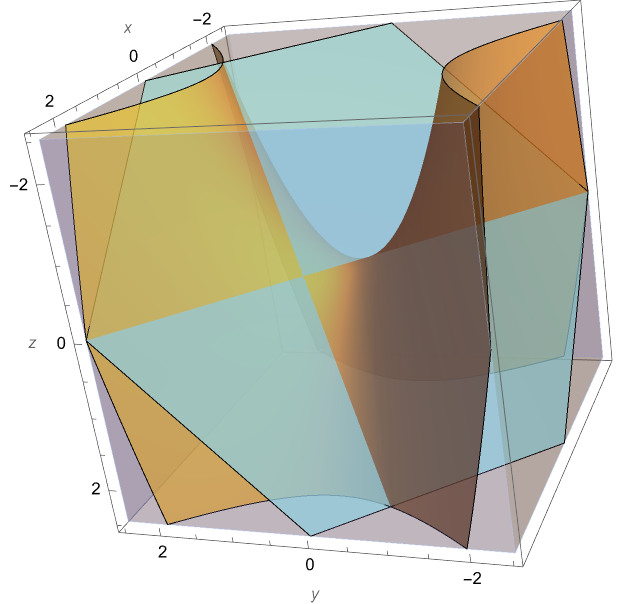
\includegraphics[width = 8cm]{weekly/week 15/Diagrams/ahoy.png}
        \hspace{2em}
        \label{fig:hyperbolic_surface}
    \end{figure}
    
    \begin{enumerate}
        \item We say a line is on the surface $S$ if every point on said line lies on $S$. See the above diagram for an example. Prove that for every point $P$ on the surface $S$, we can find exactly two lines lying on $S$ that pass through $P$.
        \item When will both of these lines be perpendicular?
    \end{enumerate}
\end{enumerate}

\newpage
\section{Combinatorics}
\begin{enumerate}[label=\textbf{C\arabic*}.]
    \item \textbf{Egregiously Messy Jumps} \newline
    Suppose we have $4$ frogs each positioned at the corners of a square of side length $1$. Every move, one of the frogs jumps over one of the other frogs, landing an equal distance of away on the opposite side.
    
    \begin{enumerate}
        \item (\fullchili) Is it possible for the frogs to end up at the vertices of a square with side length greater than $1$?
        
        \item (\fullchili \hspace{1pt} $\times$ Open)\footnote{not sure if this is open tbh, i just didn't try enough.} Suppose we have $n$ frogs on a unit side length regular $n$-sided polygon. Following the same jumping pattern, is it possible for our frogs to end up on the vertices of a regular $n$-sided polygon with a side length greater than $1$?
    \end{enumerate}
    
    \item \textbf{Unfairness}\footnote{i suck at puns} \newline
    For which $n$ is it possible to arrange the numbers $1, 2, \dots, n$ such that the average of any two numbers never lies between them?
    
\end{enumerate}

\newpage
\section{Geometry}
\begin{enumerate}[label=\textbf{G\arabic*}.]
    \item \textbf{Fair Cake-Cutting (disputen't)} \newline
    Consider a cake in the shape of a polyhedron, $P$. The cake (with volume $V$) is entirely covered in frosting (equal to surface area $A$). Suppose we wish to split the cake with planar cuts between $n$ people such that everyone receives an equal amount of cake and frosting. For which $n$ is this possible?
    
    \begin{enumerate}
        \item Consider the 2-dimensional case of this problem first. For any shape of cake $P$, we let the frosting be the perimeter. Show that, with one straight slice, we can separate two equal and fair portions of cake and frosting.
        
        \item (\fullchili) For the original problem, show that we can slice the cake into two portions of equal cake and frosting with one planar slice.
        
        \item Come up with an example that proves we cannot always produce three portions of equal cake and frosting in two planar slices.
    \end{enumerate}
\end{enumerate}

\newpage
\section{Number Theory}
\begin{enumerate}[label=\textbf{N\arabic*}.]
    \item \textbf{Forced Reality\footnote{again, this is a horrible pun. blame the 11pm brain}}
    \begin{enumerate}
        \item Suppose we have a complex number $z$ where $|z| = 1$. Prove that
        \[ \frac{z^n}{1 + z^{2n}} \]
        is real for all choices of positive integers $n$.
        
        \item (\halfchili) In addition to the above, provide a geometric proof on why the number must be real.
    \end{enumerate}
\end{enumerate}

\end{document}
